%% Adaptado de 
%% http://www.ctan.org/tex-archive/macros/latex/contrib/IEEEtran/
%% Traduzido para o congresso de IC da USP
%%*****************************************************************************
% Não modificar

\documentclass[twoside,conference,a4paper]{IEEEtran}

%******************************************************************************
% Não modificar
\usepackage{IEEEtsup} % Definições complementares e modificações.

\usepackage[english,brazil]{babel}
\usepackage[utf8]{inputenc}

%% \usepackage{latexsym,amsfonts} % Disponibiliza fontes adicionais.

\usepackage[T1]{fontenc}
\usepackage{fbb}

\usepackage{animate}

\usepackage{theorem} 
%% \usepackage[cmex10]{amsmath} % Pacote matemático básico 
\usepackage{url} 
\usepackage{graphicx}
\usepackage{amsmath}
\usepackage{amssymb}
\usepackage{color}
\usepackage[pagebackref=true,breaklinks=true,colorlinks,bookmarks=false]{hyperref}
\usepackage[tight,footnotesize]{subfigure} 
\usepackage[noadjust]{cite} % Disponibiliza melhorias em citações.
%%*****************************************************************************

\begin{document}
\selectlanguage{brazil}
\renewcommand{\IEEEkeywordsname}{Palavras-chave}

%%*****************************************************************************

\urlstyle{tt}
% Indicar o nome do autor e o curso/nível (grad-mestrado-doutorado-especial)
\title{Algoritmos Genéticos + Redes Neurais = <3}
\author{%
 \IEEEauthorblockN{João Vitor Araki Gonçalves\,\IEEEauthorrefmark{1}}
 \IEEEauthorblockN{Lucy Miyuki Miyagusiku Narita\,\IEEEauthorrefmark{2}}
 \IEEEauthorblockA{Ciência da Computação - Graduação \\
                   \IEEEauthorrefmark{1}%
                   ra176353@students.ic.unicamp.br\\
                   \IEEEauthorrefmark{2}%
                   ra182851@students.ic.unicamp.br}
}

%%*****************************************************************************

\maketitle

%%*****************************************************************************
% Modifique as seções de acordo com o seu projeto

\section{Introdução}

Este trabalho tem como objetivo implementar e aplicar uma técnica de computação evolutiva na prática.
Algoritmos genéticos problemas são resolvidos através de um processo evolutivo que resulta na solução mais adequada dado algum critério, são, portanto, muito utilizados para problemas de otimização e de busca onde o crescimento exponencial das combinações faz de um algoritmo tradicional de busca inviável.

\section{Dependências}

O projeto foi desenvolvido em Python 3.X. As dependências se encontram no arquivo \texttt{requirements.txt}.

Utilizamos o python, pois a biblioteca utilizada para \emph{deeplearning} foi o \emph{tensorflow}, e não haveria vantagem em implementar o algorítmo genético em outra linguagem, aumentando a complexidade do projeto e exigindo uma interface entre o python e uma outra linguagem qualquer.
\section{Trabalho Proposto}

As redes neurais são o ponto central da revolução do \emph{Deep Learning}. A tecnologia avançou a ponto de ser capaz de sintetizar voz, reconhecer imagens e alterar o conteúdo de videos de forma a adulterar a informação passada originalmente.

Para este projeto, procuramos fazer o \emph{tunning} dos parâmetros de uma rede neural, ou habitualmente conhecidos \emph{hyper parameters}, com um algoritmo genético. Trabalho que normalmente é feito "à mão" com base em experimentação e determinação destes valores de forma empírica.

O algorítmo foi implementado de forma genérica, sendo possível utilizá-lo com entradas genéricas, desde que sejam especificados as formas de \emph{crossover} e \emph{mutação} específicas para o problema que se deseja resolver.



\subsection{Indivíduo (Cromossomo)}

Nosso indivíduo é composto por 4 valores reais:

\begin{itemize}
    \item número de epochs
    \item quantidade de layers
    \item output space dimension para cada layer
    \item número de features
\end{itemize}

A função de \emph{fitness} foi dada pelo inverso da função de perda da rede.

\subsection{Redes Treinadas}
Para testar a aplicação de algorítmos genéticos na otimização de \emph{hyper parameters}, aplicamos o processo em três tipos de redes diferentes. Uma rede classificadora do problema \emph{MNIST}, um \emph{deep autoencoder} também para a base \emph{MNIST}. Finalmente tentamos utilizar o mesmo processo numa rede mais complexa de \emph{autoencoder} de rostos.

Devido à questões de tempo de execução, só pudemos realizar testes profundos com a rede mais simples \emph{MNIST}, que apesar de ser realativamente fácil de se obter bons resultados independente dos \emph{hyper parameters} é possível observar melhoras nos resultados utilizando o algorítmo genético.


\section{Resultados}

\subsection{MNIST}

\subsubsection{Configuração 1}

\begin{itemize}
    \item tamanho da população: 5
    \item gerações (max): 100
    \item taxa de mutação: 0.2
    \item taxa de crossover: 0.6
    \item técnica de seleção: a melhor metade da população
    \item técnica de crossover: aleatóriamente seleciona um ou mais alelos para fazer o crossover
    \begin{itemize}
        \item \emph{layers}: troca para a quantidade de layers do companheiro e anexa ou remove dados da lista de \emph{neurons} conforme necessário.
        \item \emph{neurons}: gera 2 índices aleatórios dentro da menor quantidade de \emph{neurons} entre os dois indivíduos e faz a troca entre os \emph{neurons} dos indivíduos que se encontram entre os 2 índices gerados.
        \item \emph{features}: troca para a quantidade de features do companheiro
    \end{itemize}
    \item técnica de mutação: aleatóriamente seleciona um ou mais alelos para mutar, baseando-se na taxa de mutação dos alelos.
    \begin{itemize}
        \item \emph{layers}: gera um número aleatório e duplica ou remove dados da lista de \emph{neurons} conforme necessário.
        \item \emph{neurons}: gera um novo número aleatório dentro do conjunto de valores válidos
        \item \emph{features}: gera um novo número aleatório dentro do conjunto de valores válidos
    \end{itemize}
    \item epochs: 4
    \item layers: [1-4]
    \item neurons: [100-2000]
    \item features: [1-100]
    \item critério de parada: limite de gerações atingido
    \item loss: Figura \ref{fig:loss_mnist_01}
    \item \textbf{melhor indivíduo}: Layers: 3, Neurons: [434 396 410], \# Features: 36, Loss: 0.06390089303823188
\end{itemize}

\begin{figure}[htbp]
        \centering 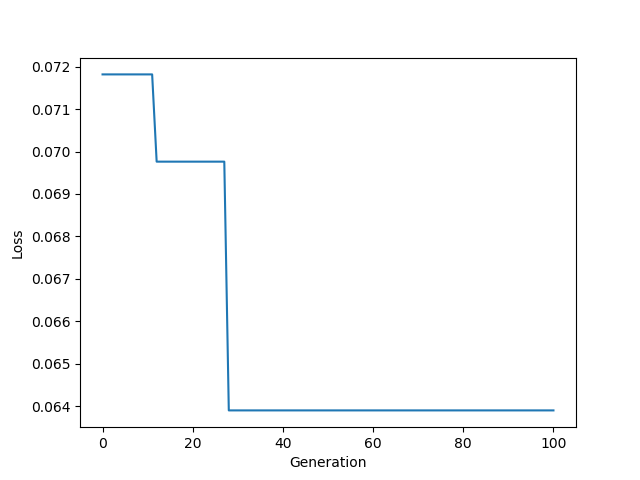
\includegraphics[width=1\columnwidth]{./ia_proj_images/mnist/1/loss.png}
        \caption{
                \label{fig:loss_mnist_01}
                Loss
        }
\end{figure}

\subsubsection{Configuração 2}

\begin{itemize}
    \item tamanho da população: 10
    \item gerações (max): 100
    \item taxa de mutação: 0.2
    \item taxa de crossover: 0.6
    \item técnica de seleção: a melhor metade da população
    \item técnica de crossover: aleatóriamente seleciona um ou mais alelos para fazer o crossover
    \begin{itemize}
        \item \emph{layers}: troca para a quantidade de layers do companheiro e anexa ou remove dados da lista de \emph{neurons} conforme necessário.
        \item \emph{neurons}: gera 2 índices aleatórios dentro da menor quantidade de \emph{neurons} entre os dois indivíduos e faz a troca entre os \emph{neurons} dos indivíduos que se encontram entre os 2 índices gerados.
        \item \emph{features}: troca para a quantidade de features do companheiro
        \item \emph{epochs}: troca para a quantidade de epochs do companheiro
    \end{itemize}
    \item técnica de mutação: aleatóriamente seleciona um ou mais alelos para mutar, baseando-se na taxa de mutação dos alelos.
    \begin{itemize}
        \item \emph{layers}: gera um número aleatório e duplica ou remove dados da lista de \emph{neurons} conforme necessário.
        \item \emph{neurons}: gera um novo número aleatório dentro do conjunto de valores válidos
        \item \emph{features}: gera um novo número aleatório dentro do conjunto de valores válidos
        \item \emph{epochs}: gera um novo número aleatório dentro do conjunto de valores válidos
    \end{itemize}
    \item epochs: [1-10]
    \item layers: [1-4]
    \item neurons: [100-2000]
    \item features: [1-100]
    \item critério de parada: limite de gerações atingido
    \item loss: Figura \ref{fig:loss_mnist_02}
    \item accuracy: Figura \ref{fig:acc_mnist_02}
    \item \textbf{melhor indivíduo}: Layers: 3, Neurons: [219  12 182], Loss: 0.06365562731241807, Epochs: 7
\end{itemize}

\begin{figure}[htbp]
        \centering 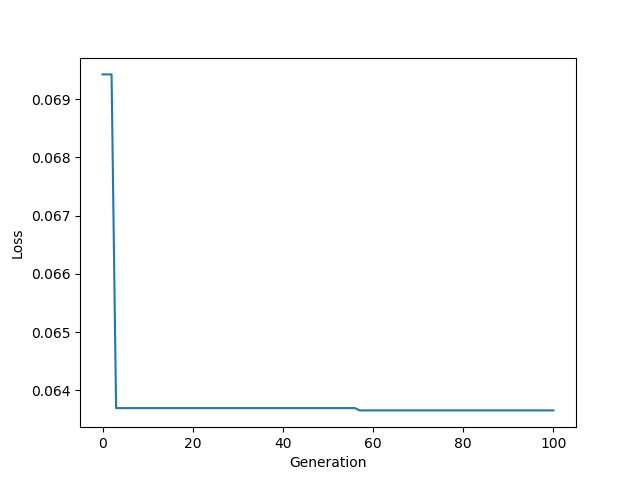
\includegraphics[width=1\columnwidth]{./ia_proj_images/mnist/2/loss.png}
        \caption{
                \label{fig:loss_mnist_02}
                Loss
        }
\end{figure}
\begin{figure}[htbp]
        \centering 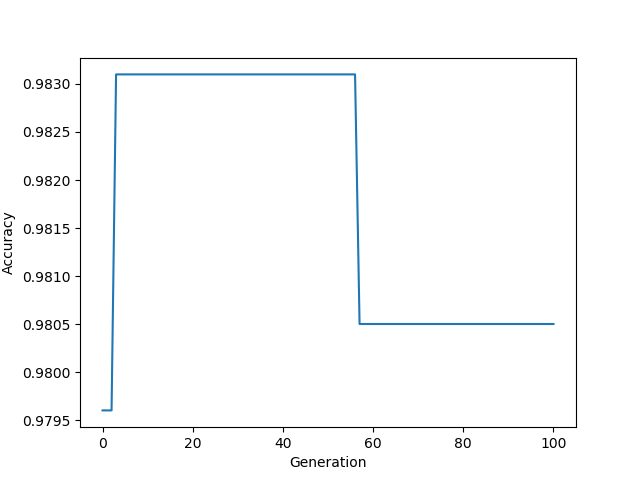
\includegraphics[width=1\columnwidth]{./ia_proj_images/mnist/2/acc.png}
        \caption{
                \label{fig:acc_mnist_02}
                Accuracy
        }
\end{figure}

\subsubsection{Configuração 3}

\begin{itemize}
    \item tamanho da população: 10
    \item gerações (max): 100
    \item taxa de mutação: 0.7
    \item taxa de crossover: 0.8
    \item técnica de seleção: a melhor metade da população
    \item técnica de crossover: aleatóriamente seleciona um ou mais alelos para fazer o crossover
    \begin{itemize}
        \item \emph{neurons}: troca o último valor entre os indivíduos
        \item \emph{epochs}: troca para a quantidade de epochs do companheiro
    \end{itemize}
    \item técnica de mutação: aleatóriamente seleciona um ou mais alelos para mutar, baseando-se na taxa de mutação dos alelos.
    \begin{itemize}
        \item \emph{layers}: gera um número aleatório e duplica ou remove dados da lista de \emph{neurons} conforme necessário.
        \item \emph{neurons}: gera um novo número aleatório (distribuição uniforme) dentro do conjunto de valores válidos
        \item \emph{epochs}: gera um novo número aleatório (distribuição uniforme) dentro do conjunto de valores válidos
    \end{itemize}
    \item epochs: [1-10]
    \item layers: [1-4]
    \item neurons: [100-2000]
    \item features: [1-100]
    \item critério de parada: limite de gerações atingido
    \item loss: Figura \ref{fig:loss_mnist_03}
    \item accuracy: Figura \ref{fig:acc_mnist_03}
    \item \textbf{melhor indivíduo}: Layers: 3, Neurons: [466 137 334], Loss: 0.060888413391448556, Epochs: 4
\end{itemize}

\begin{figure}[htbp]
        \centering 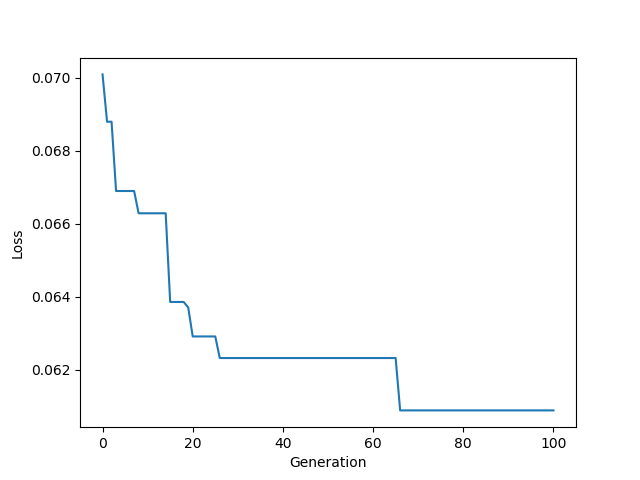
\includegraphics[width=1\columnwidth]{./ia_proj_images/mnist/3/loss.png}
        \caption{
                \label{fig:loss_mnist_03}
                Loss
        }
\end{figure}
\begin{figure}[htbp]
        \centering 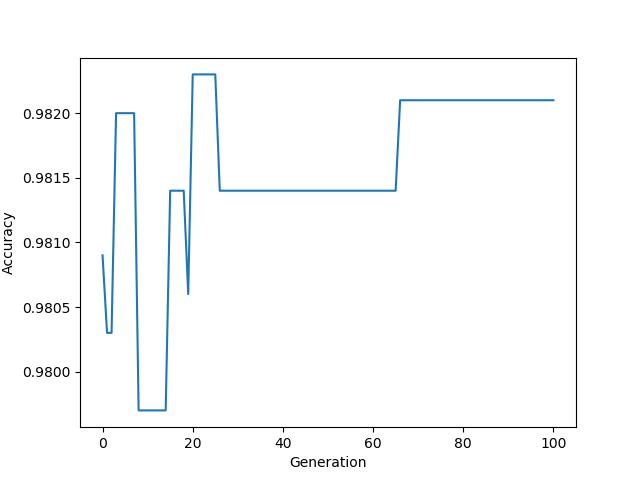
\includegraphics[width=1\columnwidth]{./ia_proj_images/mnist/3/acc.png}
        \caption{
                \label{fig:acc_mnist_03}
                Accuracy
        }
\end{figure}

\subsubsection{Configuração 4}

\begin{itemize}
    \item tamanho da população: 5
    \item gerações (max): 100
    \item taxa de mutação: 0.7
    \item taxa de crossover: 0.8
    \item técnica de seleção: a melhor metade da população
    \item técnica de crossover: aleatóriamente seleciona um ou mais alelos para fazer o crossover
    \begin{itemize}
        \item \emph{neurons}: troca o último valor entre os indivíduos
        \item \emph{epochs}: troca para a quantidade de epochs do companheiro
    \end{itemize}
    \item técnica de mutação: aleatóriamente seleciona um ou mais alelos para mutar, baseando-se na taxa de mutação dos alelos.
    \begin{itemize}
        \item \emph{layers}: gera um número aleatório e duplica ou remove dados da lista de \emph{neurons} conforme necessário.
        \item \emph{neurons}: gera um novo número aleatório (distribuição uniforme) dentro do conjunto de valores válidos
        \item \emph{epochs}: gera um novo número aleatório (distribuição uniforme) dentro do conjunto de valores válidos
    \end{itemize}
    \item epochs: 5
    \item layers: [1-4]
    \item neurons: [100-2000]
    \item features: [1-100]
    \item critério de parada: limite de gerações atingido
    \item loss: Figura \ref{fig:loss_mnist_04}
    \item accuracy: Figura \ref{fig:acc_mnist_04}
    \item \textbf{melhor indivíduo}: Layers: 2, Neurons: [467.68464507  88.63032893], Loss: 0.05897278582537547, Epochs: 5
\end{itemize}

\begin{figure}[htbp]
        \centering 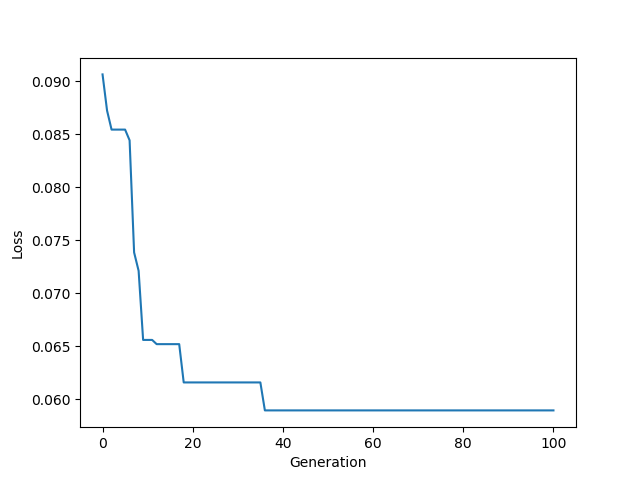
\includegraphics[width=1\columnwidth]{./ia_proj_images/mnist/4/loss.png}
        \caption{
                \label{fig:loss_mnist_04}
                Loss
        }
\end{figure}
\begin{figure}[htbp]
        \centering 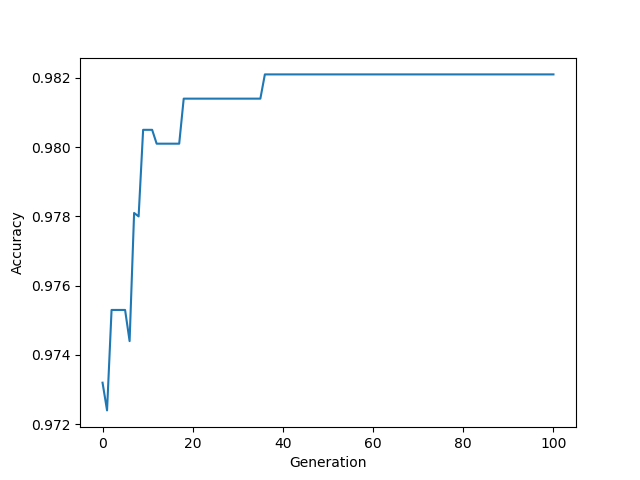
\includegraphics[width=1\columnwidth]{./ia_proj_images/mnist/4/acc.png}
        \caption{
                \label{fig:acc_mnist_04}
                Accuracy
        }
\end{figure}

\subsubsection{Configuração 5}

\begin{itemize}
    \item tamanho da população: 5
    \item gerações (max): 100
    \item taxa de mutação: 0.7
    \item taxa de crossover: 0.8
    \item técnica de seleção: a melhor metade da população
    \item técnica de crossover: aleatóriamente seleciona um ou mais alelos para fazer o crossover
    \begin{itemize}
        \item \emph{neurons}: troca o último valor entre os indivíduos
        \item \emph{epochs}: troca para a quantidade de epochs do companheiro
    \end{itemize}
    \item técnica de mutação: aleatóriamente seleciona um ou mais alelos para mutar, baseando-se na taxa de mutação dos alelos.
    \begin{itemize}
        \item \emph{layers}: gera um número aleatório e duplica ou remove dados da lista de \emph{neurons} conforme necessário.
        \item \emph{neurons}: gera um novo número aleatório (distribuição uniforme) dentro do conjunto de valores válidos
        \item \emph{epochs}: gera um novo número aleatório (distribuição uniforme) dentro do conjunto de valores válidos
    \end{itemize}
    \item epochs: [1-10]
    \item layers: [1-4]
    \item neurons: [100-2000]
    \item features: [1-100]
    \item critério de parada: limite de gerações atingido
    \item loss: Figura \ref{fig:loss_mnist_05}
    \item accuracy: Figura \ref{fig:acc_mnist_05}
    \item \textbf{melhor indivíduo}: Layers: 2, Neurons: [467.68464507  88.63032893], Loss: 0.05897278582537547, Epochs: 5
\end{itemize}

\begin{figure}[htbp]
        \centering 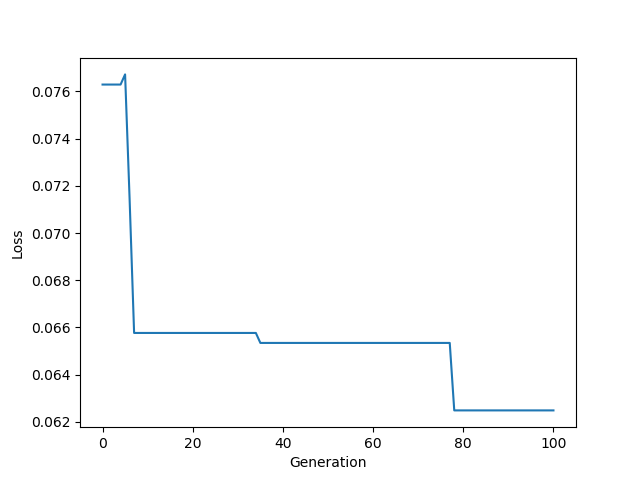
\includegraphics[width=1\columnwidth]{./ia_proj_images/mnist/5/loss.png}
        \caption{
                \label{fig:loss_mnist_05}
                Loss
        }
\end{figure}
\begin{figure}[htbp]
        \centering 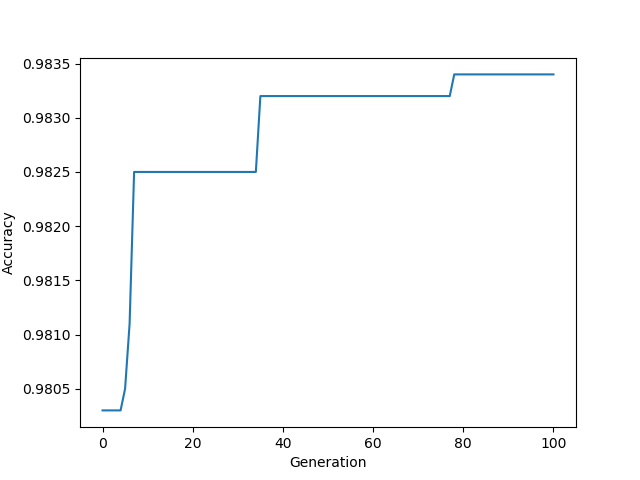
\includegraphics[width=1\columnwidth]{./ia_proj_images/mnist/5/acc.png}
        \caption{
                \label{fig:acc_mnist_05}
                Accuracy
        }
\end{figure}

\subsubsection{Configuração 6}

\begin{itemize}
    \item tamanho da população: 5
    \item gerações (max): 100
    \item taxa de mutação: 0.7
    \item taxa de crossover: 0.8
    \item técnica de seleção: toda a população
    \item técnica de crossover: aleatóriamente seleciona um ou mais alelos para fazer o crossover
    \begin{itemize}
        \item \emph{neurons}: troca o último valor entre os indivíduos
        \item \emph{epochs}: troca para a quantidade de epochs do companheiro
    \end{itemize}
    \item técnica de mutação: aleatóriamente seleciona um ou mais alelos para mutar, baseando-se na taxa de mutação dos alelos.
    \begin{itemize}
        \item \emph{layers}: gera um número aleatório e duplica ou remove dados da lista de \emph{neurons} conforme necessário.
        \item \emph{neurons}: gera um novo número aleatório (distribuição uniforme) dentro do conjunto de valores válidos
        \item \emph{epochs}: gera um novo número aleatório (distribuição uniforme) dentro do conjunto de valores válidos
    \end{itemize}
    \item epochs: [1-10]
    \item layers: [1-4]
    \item neurons: [100-2000]
    \item features: [1-100]
    \item critério de parada: limite de gerações atingido
    \item loss: Figura \ref{fig:loss_mnist_06}
    \item accuracy: Figura \ref{fig:acc_mnist_06}
    \item \textbf{melhor indivíduo}: Layers: 3, Neurons: [465.81245762 328.73175283 328.73175283], Loss: 0.05875796907646581, Epochs: 5, Acc: 0.9825000166893005
\end{itemize}

\begin{figure}[htbp]
        \centering 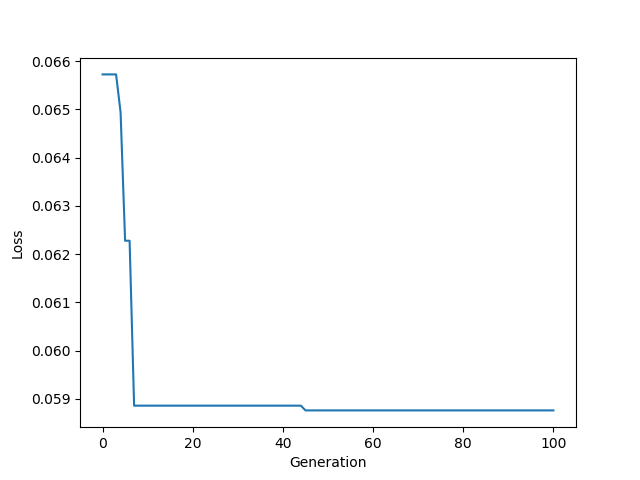
\includegraphics[width=1\columnwidth]{./ia_proj_images/mnist/6/loss.png}
        \caption{
                \label{fig:loss_mnist_06}
                Loss
        }
\end{figure}
\begin{figure}[htbp]
        \centering 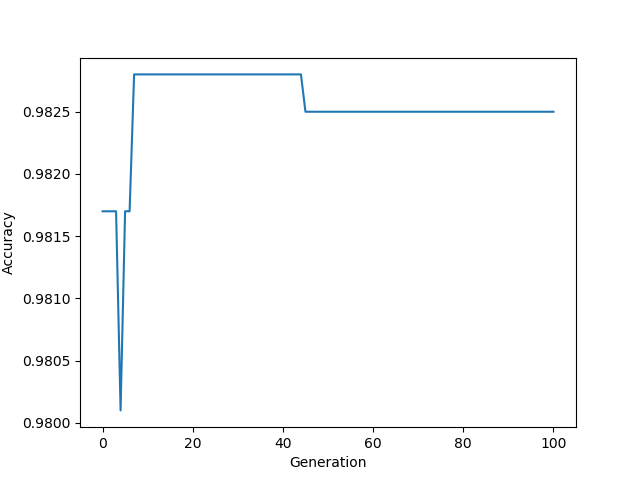
\includegraphics[width=1\columnwidth]{./ia_proj_images/mnist/6/acc.png}
        \caption{
                \label{fig:acc_mnist_06}
                Accuracy
        }
\end{figure}

\subsubsection{Configuração 7}

\begin{itemize}
    \item tamanho da população: 5
    \item gerações (max): 100
    \item taxa de mutação: 0.7
    \item taxa de crossover: 0.8
    \item técnica de seleção: toda a população
    \item técnica de crossover: aleatóriamente seleciona um ou mais alelos para fazer o crossover
    \begin{itemize}
        \item \emph{neurons}: troca o último valor entre os indivíduos
        \item \emph{epochs}: troca para a quantidade de epochs do companheiro
    \end{itemize}
    \item técnica de mutação: aleatóriamente seleciona um ou mais alelos para mutar, baseando-se na taxa de mutação dos alelos.
    \begin{itemize}
        \item \emph{layers}: gera um número aleatório e duplica ou remove dados da lista de \emph{neurons} conforme necessário.
        \item \emph{neurons}: gera um novo número aleatório (distribuição uniforme) dentro do conjunto de valores válidos
        \item \emph{epochs}: gera um novo número aleatório (distribuição uniforme) dentro do conjunto de valores válidos
    \end{itemize}
    \item epochs: [1-10]
    \item layers: [1-4]
    \item neurons: [100-2000]
    \item features: [1-100]
    \item critério de parada: limite de gerações atingidos \textbf{ou} sem variação por 20 gerações
    \item loss: Figura \ref{fig:loss_mnist_07}
    \item accuracy: Figura \ref{fig:acc_mnist_07}
    \item \textbf{melhor indivíduo}: Layers: 2, Neurons: [460.28380887 221.80215432], Loss: 0.06304866494573652, Epochs: 4, Acc: 0.9815999865531921
\end{itemize}

\begin{figure}[htbp]
        \centering 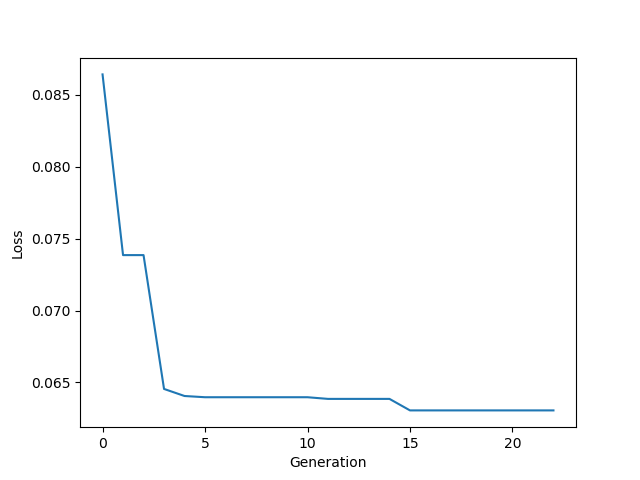
\includegraphics[width=1\columnwidth]{./ia_proj_images/mnist/7/loss.png}
        \caption{
                \label{fig:loss_mnist_07}
                Loss
        }
\end{figure}
\begin{figure}[htbp]
        \centering 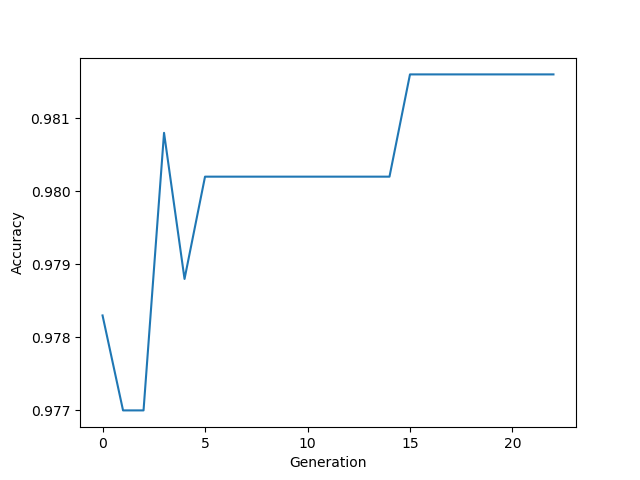
\includegraphics[width=1\columnwidth]{./ia_proj_images/mnist/7/acc.png}
        \caption{
                \label{fig:acc_mnist_07}
                Accuracy
        }
\end{figure}

\subsection{Autoencoder MNIST}

\begin{figure}[htbp]
        \centering 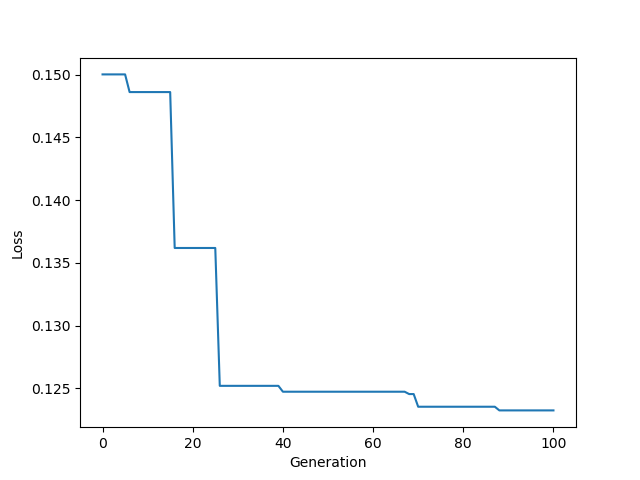
\includegraphics[width=1\columnwidth]{./ia_proj_images/mnist_auto_encoder/config_inicial_fixed_epochs_loss.png}
        \caption{
                \label{fig:loss_mnist_autoencoder}
                Loss
        }
\end{figure}

\subsection{Face Autoencoder}


\begin{figure}[htbp]
        \centering 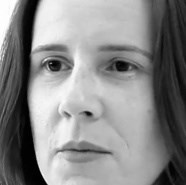
\includegraphics[width=.7\columnwidth]{./ia_proj_images/faces_auto_encoder/esther.jpg}
        \caption{
                \label{fig:esther}
                Input
        }
\end{figure}


\begin{figure}[htbp]
        \centering 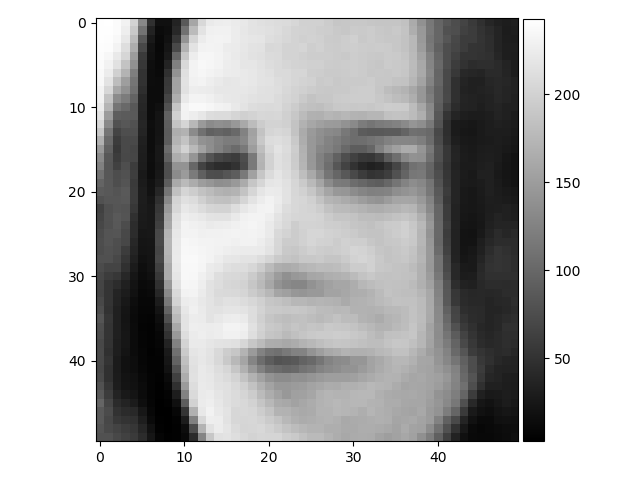
\includegraphics[width=1\columnwidth]{./ia_proj_images/faces_auto_encoder/esther_auto.png}
        \caption{
                \label{fig:esther_auto}
                Output
        }
\end{figure}

\begin{figure}[htbp]
        \centering 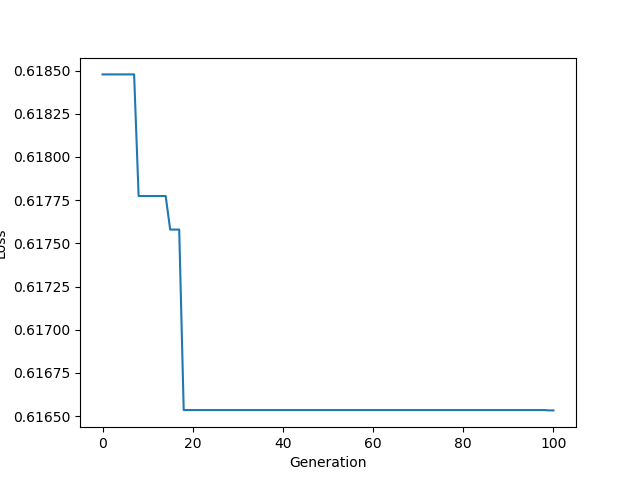
\includegraphics[width=1\columnwidth]{./ia_proj_images/faces_auto_encoder/loss.png}
        \caption{
                \label{fig:loss_esther}
                Loss
        }
\end{figure}

\section{Discussão}
Em relação aos testes realizados com a rede \emph{MNIST}:
Em todas as configurações, pode-se observar uma melhora do decorrer da execução das gerações, principalmente a configuração \emph{7} que obteve o melhor resultado de todas.
Podemos realizar a seguinte discussão em relação às configurações encontradas como melhores para esse algorítmo genético.

\begin{itemize}
    \item \emph{tamanho da população}: uma população de 5 indivíduos apresentou o melhor resultado, além de ser duas vezes mais rápido de executar, convergiu só um pouco depois da sua versão com 10 indivíduos, em nosso caso onde paralelização não é uma opção, uma população menor apresentou melhores resultados.
    \item \emph{critério de parada}: realizamos testes com critério de parada onde se o fitness não melhorasse por 20 gerações, o treino é interrompido. Porém observando os gráficos, temos períodos de quase 50 gerações sem melhoras, para então uma melhora significativa dos resultados. Então para evitar perdas, mantivemos o número de gerações fixas em 100, que é aproximadamente o máximo que podemos razoávelmente manter executando (apróxidamente 2h de execução para às 100 gerações)
    \item \emph{técnica de seleção}: Antes era feita a a seleção de apenas metade dos melhores indivíduos para reprodução, observamos que obtivemos resultados melhores selecionando \emph{todos} os indivíduos. Isso pode-se explicar pelo fato de que temos poucos indivíduos na população, metade deles são apenas dois, que torda a progressão bem lenta por mutações aleatórias, com todos os 5 selecionados, obtivemos melhores soluções mais rápido.
    \item técnica de crossover
    \item técnica de mutação
    \item método de substituição
    \item taxa de mutação
    \item taxa de crossover
\end{itemize}

Nas diferentes configurações, testamos duas funções de fitness, uma minimizando a função de \emph{loss} da rede e uma otimizando a métrica de \emph{accuracy}, optamos por fazer a maioria dos testes minimizando o \emph{loss} já que no geral, quanto menor o loss melhor é a accuracy, e o teste maximizando a accuracy não forneceu os melhores resultados.

Outra alteração foi a adição do núemro de epochs no cromossomo, que inicialmente era uma valor fixo (4). Isso se deu ao fato de que as redes estavam ficando limitadas pelo o núemro de epochs, já que uma rede pequena sofre overfitting em 4 epochs e uma grande não treina adequadamente. Por isso o número de epochs que a rede treina se tornou outro parâmetro do indivíduo, que trouxe resultados melhores. \\

Agora uma breve discussão sobre as redes autoencoder testadas. 

Primeiramente sobre o autoencoder \emph{MNIST}: Obtivemos resultados bons com os testes iniciais com essa rede, porém o tempo para executar todas as 100 gerações do algorítmo genético se mostrou proibitivo para realizar testes com outras configurações, então esse caso fica apenas como prova de que essa técnica pode ser utilizada em diferentes tipos de redes neurais, não apenas redes classificadoras simples.

Finalmente sobre o autoencoder de rostos: Essa rede foi a que demandou o maior esforço para configuração inicial. Foi necessário fazer crawling de 40 mil fotos de rostos de artistas na internet, e pré-processar todas elas com um algorítmo de centralização de rostos. Infelizmente, essa rede se mostrou mais demorada para se treinar que o esperado, para treinar a rede até resultados satisfatórios, foi necessário treina-la por um total de 8 horas. Esse seria o tempo para executar a função de fitness de um único indivíduo no algorítmo genético, claramente algo proibitivo. Como forma de conceito fizemos um teste treinando cada rede um total de 2 minutos (muito longe de se obter resultados razoáveis), e é possível observar uma melhora no resultado obtido, então teoricamente, se tivéssemos o tempo hábil e recursos, seria possível otimizar toda a rede para \emph{hyper parameters} ideais.


Outro ponto é que esse projeto não seria possível sem acesso à uma \emph{GPU} para acelerar o treino das redes. O tempo de execução numa \emph{GTX 970} foi de 1 hora e 30 minutos no total para cada configuração, e teria durado um total de 4 horas caso fosse executada somente na \emph{CPU} (no caso um \emph{i7 4790k}), o que inviabilizaria as análises necessárias pelo projeto.

\section{Conclusões}

Tivemos alguns problemas no decorrer do projeto por conta do tempo gasto como treinamento da rede para cada indivíduo gerado pelo algoritmo genético, além disso, alguns de nossos resultados (autoencoder de rostos) não foram tão bem sucedidos quanto esperado.

Então com recursos limitados e redes mais complexas, um algorítmo genético não é uma opção viável, já que o poder de processamento necessário é alto demais para viabilizar essa abordagem. Porém se recursos não são um problema, e devido ao fato do algorítmo genético ser fácilmente paralelizável portanto escalável, e se ter o melhor resultado possível da rede é uma prioridade, então algorítmos genéticos são um bom caminho para a definição de \emph{hyper parameters}. 

Ainda sim, gostaríamos de argumentar que o projeto pode ser considerado um sucesso no que se refere ao seu objetivo principal: implementar, aplicar e analisar os resultados obtidos através de um algoritmo genético aplicado a um problema real ou da literatura.



%******************************************************************************
% Referências - Definidas no arquivo Relatorio.bib
%  +----------------+

% \bibliographystyle{IEEEtran}

% \bibliography{Relatorio}


%******************************************************************************


\end{document}
